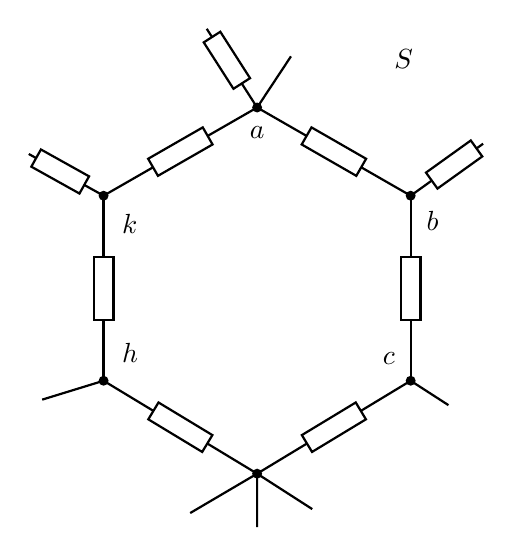
\begin{tikzpicture}[x=1cm,y=1cm,line width=0.8pt]
  \coordinate (a) at (0,2.35);
  \coordinate (b) at (1.95,1.23);
  \coordinate (c) at (1.95,-1.12);
  \coordinate (m) at (0,-2.30);
  \coordinate (h) at (-1.95,-1.12);
  \coordinate (k) at (-1.95,1.23);

  % The unlabelled lower vertex represents intermediate nodes in ab,bc,...,hk,ka.
  \foreach \from/\to in {a/b,b/c,c/m,m/h,h/k,k/a} {
    \draw (\from)--node[midway,sloped,draw,fill=white,
      minimum width=8mm,minimum height=2.5mm,inner sep=0pt]{} (\to);
  }

  % Other branches incident at the loop vertices remain visible.
  \draw (a)--++(0.43,0.65);
  \draw (a)--node[pos=0.60,sloped,draw,fill=white,
    minimum width=7mm,minimum height=2.5mm,inner sep=0pt]{} ++(-0.64,1.00);
  \draw (b)--node[pos=0.60,sloped,draw,fill=white,
    minimum width=7mm,minimum height=2.5mm,inner sep=0pt]{} ++(0.92,0.66);
  \draw (c)--++(0.48,-0.31);
  \draw (m)--++(-0.85,-0.50) (m)--++(0.70,-0.45) (m)--++(0,-0.68);
  \draw (h)--++(-0.78,-0.24);
  \draw (k)--node[pos=0.58,sloped,draw,fill=white,
    minimum width=7mm,minimum height=2.5mm,inner sep=0pt]{} ++(-0.95,0.53);

  \foreach \p in {a,b,c,m,h,k} {\fill (\p) circle (1.8pt);}
  \node[below=3pt] at (a) {$a$};
  \node[below right=2pt] at (b) {$b$};
  \node[above left=2pt] at (c) {$c$};
  \node[above right=3pt] at (h) {$h$};
  \node[below right=3pt] at (k) {$k$};
  \node at (1.86,2.96) {$S$};
\end{tikzpicture}
